\documentclass{optica-article}
\journal{opticajournal} % for journals or Optica Open
\articletype{Research Article}
\usepackage{lineno}
\usepackage{verbatim}
\usepackage{graphicx} %immagini ecc
\usepackage{float}
\usepackage{hyperref}
\usepackage{placeins}

\pagestyle{plain}
\begin{document}

\begin{center}
    \Huge \textbf{Relazione Tecnica}
\end{center}
\author{\centering NaoChallenge 2025}
\bigskip

\noindent
\textbf{Per ulteriori informazioni} \\

\noindent\textit{Visita il nostro sito} \href{https://www.naoartemis.altervista.org/html}{website}

\noindent\textit{Vedi la nostra} \href{https://github.com/NaoArtemis/ChallengeNao25}{repository}

\noindent\textit{Scrivi una mail a: }
\email{socialnaoartemis@gmail.com}

\bigskip

\begin{figure}
    \centering
    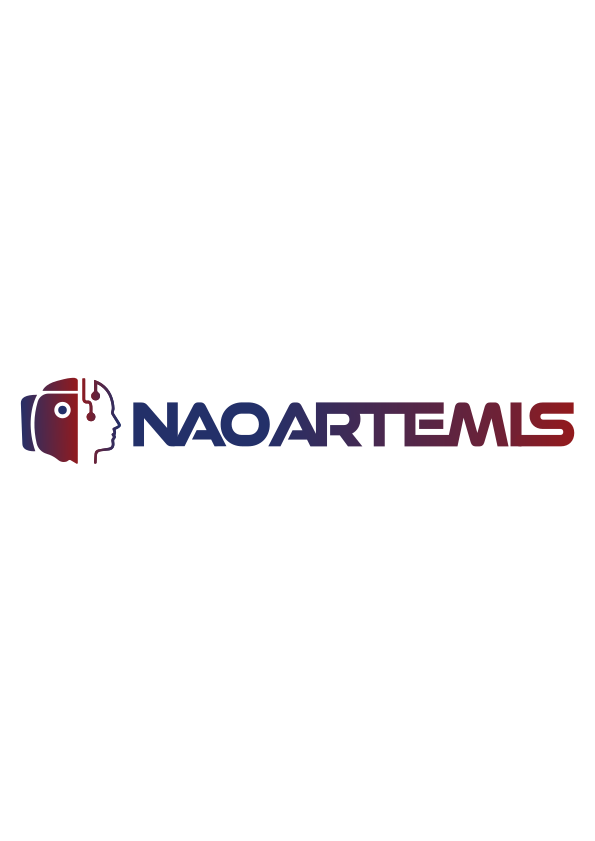
\includegraphics[scale=0.10]{figures/logo_v3.png}
    \label{fig:logo_con_scritta}
\end{figure}

\tableofcontents

\vspace{10pt}

\newpage

\begin{abstract*} 
\vspace{5pt}
\noindent

Il progetto di NaoArtemis è stato sviluppato per la NAO Challenge 2025 con l’obiettivo  di promuovere l’integrazione avanzata della tecnologia nel settore sportivo, al fine di migliorare l’esperienza sia degli atleti sia degli spettatori. La missione del progetto si fonda sull’unione tra innovazione tecnologica e inclusività, con particolare attenzione all’accessibilità e all'inclusione.

Uno degli obiettivi principali è l’ottimizzazione della preparazione atletica attraverso l’utilizzo del robot umanoide NAO. Quest’ultimo sarà in grado di monitorare i movimenti degli atleti, fornendo feedback per il miglioramento delle performance. Inoltre, verranno rilevati parametri biometrici quali la frequenza cardiaca e il numero di passi, con l’obiettivo di prevenire infortuni e supportare i processi di recupero fisico. Anche la salute mentale degli sportivi sarà oggetto di attenzione: NAO assumerà il ruolo di assistente motivazionale virtuale, offrendo rinforzi positivi e suggerimenti personalizzati.

Parallelamente, il progetto intende rendere l’esperienza sportiva più inclusiva per il pubblico, con un focus specifico sulle persone con disabilità. In particolare, NAO fornirà supporto comunicativo a persone nello spettro autistico, mediante l’adozione di sistemi di Comunicazione Aumentativa e Alternativa (CAA), favorendo così l’interazione e la partecipazione attiva agli eventi sportivi.

Infine, in collaborazione con la società sportiva Audace, il progetto prevede la sperimentazione sul campo delle soluzioni proposte, contribuendo concretamente all’innovazione del panorama sportivo attraverso l’uso della robotica e dell’intelligenza artificiale.
\vspace{5pt}
\section{Metodologia e tecniche usate}

\subsection{DevOps e metodologia Agile}
Per la gestione del progetto e il monitoraggio continuo dei progressi, il team ha adottato pratiche e strumenti in linea con i principi del paradigma DevOps (Development \& Operations), che promuove la collaborazione integrata tra sviluppo software e operazioni tecnologiche.

Lo sviluppo è stato organizzato secondo la metodologia Agile, che prevede una pianificazione iterativa e incrementale. I task principali sono stati suddivisi in sub-task, assegnati ai membri del team in base alle competenze specifiche e agli obiettivi delle singole fasi progettuali. Questo approccio ha favorito una maggiore efficienza operativa, migliorando la produttività e l'organizzazione del lavoro.

L’impiego di strumenti per la pianificazione delle attività, il monitoraggio dell’avanzamento e l’organizzazione dei flussi di lavoro ha garantito una distribuzione chiara delle responsabilità e una comunicazione efficace all’interno del gruppo di lavoro.  
Parallelamente, il progetto è stato gestito e versionato tramite \textit{GitHub}, permettendo il rilascio di diverse versioni migliorate nel tempo. 

\subsection{GitHub}
GitHub è una piattaforma cloud-based che consente la gestione distribuita del codice sorgente, favorendo la collaborazione tra sviluppatori all’interno di progetti software. Alla base di GitHub vi è Git, un sistema di versionamento distribuito che registra in modo puntuale ogni modifica apportata al codice, consentendo la gestione parallela di più versioni del progetto e prevenendo la perdita di dati.

All’interno della piattaforma, i progetti sono strutturati in repository. Gli sviluppatori possono eseguire operazioni di clonazione per ottenere copie locali dei repository, effettuare modifiche in locale, e sincronizzarle con la repository remota tramite comandi come \emph{commit} e \emph{push}.

La collaborazione tra membri del team è facilitata da strumenti avanzati come le \emph{pull request}, che permettono di proporre modifiche e sottoporle a revisione prima dell’integrazione nel branch principale, e dal sistema di \emph{issue tracking}, utile per la gestione strutturata di bug, segnalazioni e richieste di nuove funzionalità.

Per ottimizzare l'organizzazione del lavoro, il team ha adottato una struttura modulare delle repository, distinguendo due branch, uno dedicato allo sviluppo del codice (“coding”) e uno multimediale (“social”).

\subsection{File gestione presenze}
Per garantire una gestione efficace delle attività progettuali, il team NaoArtemis ha monitorato costantemente la presenza e il contributo operativo di ciascun componente attraverso un sistema tabellare condiviso che riepiloga i dati aggregati per ogni membro:
\begin{itemize}
  \item Ore lavorate complessive
  \item Numero di giorni di presenza effettiva
  \item Percentuale di partecipazione sul totale delle giornate di lavoro 
\end{itemize}

Queste informazioni sono state fondamentali per valutare l’impegno individuale e per organizzare in modo bilanciato il carico di lavoro, anche in fase di revisione delle responsabilità. Si tratta di ore PCTO (Percorsi per le Competenze Trasversali e l’Orientamento), ovvero attività obbligatorie di formazione esterna previste per gli studenti delle scuole superiori.

L’organizzazione del lavoro ha seguito un approccio ispirato al modello startup/impresa, con una gestione autonoma ed efficiente dei compiti. Questo sistema ha permesso di quantificare con precisione il contributo di ciascun membro, fornendo una base oggettiva per l’analisi dell’operatività del team e per la stesura finale della documentazione relativa alla NAO Challenge 2025.


\begin{figure}[H]
    \centering
    \includegraphics[width=0.9\textwidth]{figures/divisione_team.png}
    \caption{Tabella \texttt{DIVISIONE TEAM}: suddivisione dei membri nei rispettivi team, con indicazione del compito principale, email e numero di telefono.}
    \label{fig:divisione_team}
\end{figure}

\begin{figure}[H]
    \centering
    \includegraphics[width=0.9\textwidth]{figures/file_presenze.png}
    \caption{Tabella \texttt{PRESENZE}: registro presenze giornaliere del team per la data del 27/01/2025, con indicazione di partecipazione e team.}
    \label{fig:presenze}
\end{figure}

\bigskip

\noindent

\end{abstract*}

%%%%%%%%%%%%%%%%%%%%%%%%%%  body  %%%%%%%%%%%%%%%%%%%%%%%%%%

\section{Descrizione progetto Nao Challenge 2025}

\subsection{Dalla sfida alla realt\`a: NaoArtemis e la NAO Challenge 2025}
La NAO Challenge \`e una competizione annuale di robotica educativa rivolta a scuole secondarie, istituti tecnici, universit\`a e team di ricerca. L'obiettivo dell'iniziativa \`e promuovere l'utilizzo del robot umanoide NAO nello sviluppo di soluzioni tecnologiche innovative, capaci di rispondere a esigenze reali della societ\`a. Attraverso questa sfida, i partecipanti sono chiamati ad applicare competenze avanzate di programmazione, intelligenza artificiale, progettazione di interfacce e interazione uomo-robot in scenari pratici e multidisciplinari.

Ogni edizione della competizione \`e incentrata su un tema specifico, pensato per stimolare la creativit\`a progettuale e l'approccio ingegneristico dei team. L'edizione 2025 \`e focalizzata sullo sport: i partecipanti dovranno progettare applicazioni che utilizzino le funzionalit\`a del robot NAO per ottimizzare, personalizzare o ampliare l'esperienza sportiva, sia dal punto di vista dell'atleta sia da quello del pubblico.

Il focus progettuale comprende aspetti quali il monitoraggio delle performance fisiche, il supporto all'inclusione e all'accessibilit\`a, e l'utilizzo della robotica per migliorare l'engagement e la fruizione dello sport. Partecipare alla NAO Challenge significa affrontare un contesto competitivo ad alto contenuto tecnologico, in cui \`e fondamentale integrare competenze tecniche con sensibilit\`a verso tematiche sociali e di impatto.

\subsection{Significato del nome \text{NAO Coach \& Care (NC\&C)}}

Il nome \text{NAO Coach \& Care}, abbreviato in \text{NC\&C}, rappresenta in modo sintetico ed efficace la doppia finalità del nostro progetto per la NAO Challenge 2025. 

Da un lato, il termine \textit{Coach} evidenzia il ruolo del robot NAO come assistente tecnico per l’allenatore, capace di supportare l’analisi tattica e fisica durante le partite e gli allenamenti. Dall’altro, il termine \textit{Care} richiama la componente inclusiva del progetto, che mira a migliorare l’accessibilità sugli spalti per persone nello spettro autistico, grazie al supporto del robot e all’uso della Comunicazione Aumentativa e Alternativa (CAA).


\subsection{Audace al fianco di NaoArtemis 2025}
Audace Calcio a 5 Femminile, una delle realt\`a sportive pi\`u consolidate e innovative del panorama veronese, \`e sponsor ufficiale del progetto NaoArtemis per l'edizione 2025 della NAO Challenge. Il club si distingue a livello nazionale per l'eccellenza nei risultati sportivi e per l'approccio multidimensionale alla preparazione atletica, con un focus costante sul benessere fisico e mentale delle proprie atlete.

La collaborazione tra Audace e il team NaoArtemis nasce da una visione condivisa che pone al centro l'innovazione tecnologica applicata allo sport, l'inclusivit\`a e la promozione del talento giovanile. In particolare, il supporto di Audace ha permesso di testare in un contesto reale le soluzioni sviluppate nel progetto, che integrano robotica e intelligenza artificiale a beneficio della performance, della prevenzione degli infortuni e dell'accessibilit\`a dell'attivit\`a sportiva.

Audace si conferma cos\`i non solo come una societ\`a impegnata sul campo, ma anche come partner attivo nello sviluppo di nuove tecnologie a servizio dello sport femminile, della sostenibilit\`a e dell'inclusione. Il sostegno al progetto NaoArtemis rappresenta un ulteriore passo verso una visione dello sport come strumento evolutivo, educativo e socialmente responsabile.

\begin{figure}[H]
    \centering
    \includegraphics[width=0.6\textwidth]{figures/audace.png}
    \caption{Logo of Audace C5 Verona}
    \label{fig:audace_logo}
\end{figure}

\bigskip
\section{Task 1 -- Supporto tecnico e motivazionale agli atleti}

\subsection{Descrizione Task 1}
Il primo robot NAO sar\`a configurato per svolgere il ruolo di assistente tecnico virtuale, operando direttamente nell'area tecnica. Le sue funzioni principali includono:

\begin{itemize}
    \item \text{Tracciamento e Analisi del Movimento Sportivo}: attraverso sistemi di computer vision e tracciamento dei movimenti, il robot sarà in grado di analizzare in modo asincrono la postura e le dinamiche motorie degli atleti, elaborando i dati raccolti durante allenamenti e competizioni anche in un secondo momento. 

    \item\text{Analisi biomeccanica in tempo reale}: 
    Nel contesto del progetto, vengono acquisiti dati biometrici e biomeccanici mediante dispositivi wearable (smartwatch), includendo frequenza cardiaca (bpm), conteggio dei passi e velocità di spostamento. I dati rilevati vengono trasmessi in tempo reale e memorizzati all’interno di un database relazionale basato su \textit{PostgreSQL}, dove sono strutturati in formato tabellare per consentire operazioni di interrogazione, analisi ed elaborazione successive in ambiente software dedicato.

    \item \text{Elaborazione di dati tattici e visuali}: i dati raccolti saranno trasformati in un unico diagramma di Vornoi trasmesso sulla webapp, e saranno utilizzati per generare suggerimenti strategici personalizzati per gli allenatori, utili per studiare le partite degli avversari o gli allenamenti.
\end{itemize}

\subsection{Architettura generale del sistema}
Il sistema NaoArtemis è strutturato secondo un’architettura distribuita, composta da due server indipendenti sviluppati in ambienti Python differenti per garantire la piena compatibilità tra componenti SDK e modelli avanzati di intelligenza artificiale (AI).

\begin{itemize}
 \item Il server in Python 2 è destinato esclusivamente alla comunicazione diretta con il robot NAO, resa possibile tramite l’uso della SDK di NAOqi, che richiede un ambiente Python 2.x per l’accesso alle API di basso livello del robot. A supporto dello sviluppo, è stata costantemente consultata la documentazione ufficiale disponibile online: \url{http://doc.aldebaran.com/2-8/naoqi/index.html}.

  
  \item Il server in Python 3 ospita invece la Web Application e l’infrastruttura dedicata ai modelli AI più recenti. In questo contesto sono attivi:
  \begin{itemize}
    \item YOLO per la rilevazione e tracciamento in tempo reale di giocatori e oggetti in campo;
    \item Per ogni giocatore viene calcolato il colore medio della divisa, dopodiché l'algoritmo K-means assegna un'etichetta di squadra (ad esempio \text{rosso} o \text{blu}) in base alla somiglianza cromatica.
    \item Generazione vocale di messaggi motivazionali o comunicazioni tattiche tramite le API \text{Text-to-Speech} di \text{OpenAI};
    \item Un algoritmo per il supporto tattico destinato a suggerire strategie in tempo reale durante le fasi di gioco.
  \end{itemize}
\end{itemize}

I due server comunicano tra loro tramite interfacce TCP/IP, garantendo la sincronizzazione tra input visivi, output vocali e dati di stato degli atleti. Tale configurazione consente di superare le limitazioni di compatibilità tra il framework NAO e gli strumenti di AI moderni.

\subsection{Tecniche di Computer Vision}
Il componente "Viceallenatore" integra funzionalità di computer vision, generazione automatica di suggerimenti tattici e monitoraggio in tempo reale dei parametri di gioco.

\begin{itemize}
  \item L’analisi della scena sportiva avviene tramite un sistema basato su YOLO e K-means, i quali rilevano i giocatori e ne determinano la posizione sul campo attraverso coordinate spaziali (X, Y). 
  
  \item A differenza di una heatmap tradizionale, il sistema elabora un unico diagramma di Voronoi (Voronoi Soccer) che rappresenta lo spazio di influenza di ciascun giocatore sul campo. Questo approccio consente una visualizzazione tattica più efficace per l'allenatore, evidenziando coperture, spazi liberi e squilibri posizionali.
  
  \item I dati biometrici ricevuti dalla WebApp (battito cardiaco, numero di passi, velocità media, ecc.) vengono analizzati per valutare lo stato di forma dell’atleta. Il sistema può così suggerire in tempo reale sostituzioni strategiche, anche in risposta a condizioni critiche rilevate (affaticamento, calo di rendimento, rischio infortunio).
  
  \item Infine, un algoritmo fornisce suggerimenti tattici dinamici, adattando il gioco sulla base del comportamento avversario e della situazione in campo. Il robot NAO può poi trasmettere tali indicazioni agli atleti tramite sintesi vocale, rendendo l’interazione uomo-macchina più immediata ed efficace.
\end{itemize}

\subsection{Web Application}
La WebApp sviluppata in ambiente Python 3 è il cuore gestionale del sistema e consente il controllo dell’intera infrastruttura tramite un’interfaccia utente reattiva, accessibile via browser.

\subsubsection*{Funzionalità principali}
\begin{itemize}
  \item Gestione degli infortuni, con tracciamento delle condizioni mediche e storico sanitario di ciascun atleta;
  \item Pianificazione delle partite, calendario eventi, avvisi e statistiche pre/post-gara;
  \item Database centralizzato, che raccoglie dati biometrici, comportamentali e tecnici, resi accessibili e aggiornabili in tempo reale da ciascun modulo dell’architettura.
\end{itemize}

\begin{figure}[H]
    \centering
    \includegraphics[width=\textwidth]{figures/homescreen.png}
    \caption{Home screen della webapp \textit{Football Hub}, punto di accesso alle varie funzionalità: gestione della partita, competizione, controllo del robot tramite joystick e monitoraggio della salute.}
    \label{fig:home-screen}
\end{figure}

\begin{figure}[H]
    \centering
    \includegraphics[width=\textwidth]{figures/gestione_partita.PNG}
    \caption{Sezione “Gestione Partita” della webapp, che consente il caricamento di video per analisi tattiche.}
    \label{fig:gestione-partita}
\end{figure}

\begin{figure}[H]
  \centering
  \includegraphics[width=\textwidth]{figures/audace.jpg}
  \caption{Sezione dedicata alla giornata di campionato e ai risultati della partita dell’Audace.}
\end{figure}


\subsubsection*{Controllo manuale}
Per offrire massimo controllo e flessibilità all’utente, il team ha deciso di non adottare Choregraphe, il software ufficiale per la programmazione del robot NAO, a causa di alcune limitazioni tecniche e operative. In alternativa, è stato sviluppato un sistema di comandi manuali essenziali ma strategici, tramite la WebApp. Questo modulo consente all’utente di:

\begin{itemize}
  \item Attivare/disattivare la trasmissione video;
  \item Avviare il riconoscimento ArUco;
  \item Inviare messaggi vocali;
  \item Controllare azioni base del NAO in modo diretto e flessibile.
\end{itemize}

\subsubsection*{Appendice tecnica: componenti di elaborazione video}

\paragraph{Flusso in Python 3}
Elaborazione del flusso video registrato tramite OpenCV e decodifica dei frame JPEG. I frame vengono analizzati successivamente alla partita con modelli di visione artificiale (come YOLO e Kmeans).


\begin{figure}
\centering
\includegraphics[width=0.7\textwidth]{figures/kmeans.jpg}
\caption{Codice Python 3 per l’analisi dei frame con YOLO e clustering KMeans}
\label{fig:enter-label}s
\end{figure}

\FloatBarrier

\begin{figure}[h]
\centering
\includegraphics[width=0.7\textwidth]{figures/py3_2.jpeg}
\caption{Salvataggio dati nel database da parte dell'app}
\label{fig:py3_2}
\end{figure}


\FloatBarrier

\paragraph{Flusso in Python 2}
Acquisizione dell’immagine dalla webcam del robot NAO tramite ALVideoDevice, con parametrizzazione (fps, risoluzione, luminosità) e invio del frame in formato JPEG al server Python 3 per l’elaborazione successiva.

\begin{figure}[h]
\centering
\includegraphics[width=\textwidth]{figures/py3_1.jpeg}
\caption{Codice Python 2 che riceve un testo in ingresso e genera un file audio MP3 utilizzando la libreria OpenAI.}
\label{fig:py2}
\end{figure}
\FloatBarrier

\paragraph{Qualità video e accuratezza dell’analisi}
Durante le fasi di test, è emerso che l’utilizzo della videocamera integrata del NAO, presenta limitazioni in termini di risoluzione e qualità dell’immagine. Per questo motivo, si è scelto di sperimentare la registrazione delle partite tramite smartphone o videocamere professionali, ottenendo risultati  migliori grazie alla maggiore nitidezza e stabilità del video, che agevolano le fasi successive di analisi basata su computer vision.
\FloatBarrier

\paragraph{WebApp Flask}
Gestione delle API di autenticazione e raccolta dati biometrici tramite richieste HTTP POST da applicazione client o mobile.

\subsection{Descrizione generale dell'applicazione}
L'applicazione \`e progettata per il monitoraggio continuo e in tempo reale di parametri biometrici relativi all'attivit\`a fisica e alle condizioni fisiologiche dell'utente. Il sistema consente l'acquisizione, la trasmissione e la gestione centralizzata dei dati.

\subsection{Parametri rilevati dall'app}
\begin{itemize}
    \item \text{Numero di passi}: calcolato mediante l'utilizzo dei sensori presenti nello smartphone, in particolare accelerometro e giroscopio, che rilevano variazioni nella postura e nel movimento dell'utente. L'elaborazione avviene localmente tramite un modulo di analisi del pattern motorio.
    \item \text{Velocit\`a di movimento}: derivata dal tracciamento GPS attraverso un algoritmo che valuta la variazione di posizione rispetto al tempo, con eventuali correzioni su base temporale per compensare anomalie dovute al segnale satellitare o a cambiamenti di direzione.
    \item \text{Frequenza cardiaca (bpm)}: ottenuta da un dispositivo indossabile che comunica in modalit\`a wireless con la piattaforma Google Fit. L'applicazione si interfaccia con tale piattaforma tramite API REST, effettuando interrogazioni periodiche per la raccolta dei dati aggiornati, poi integrati nel sistema interno.
\end{itemize}

\subsection{Interfaccia utente}
All'avvio, l'applicazione presenta all'utente un'interfaccia grafica intuitiva per l'autenticazione o la registrazione, in cui vengono richiesti dati identificativi obbligatori, tra cui nome, cognome, ID giocatore univoco e password cifrata. Questi dati sono trattati in conformit\`a alle normative vigenti in materia di protezione dei dati personali con memorizzazione sicura lato server.
\begin{figure}[H]
    \centering
    \includegraphics[width=0.5\textwidth]{figures/creaaccount_app.jpg}
    \caption{Interfaccia della schermata di login}
    \label{fig:registrazione}
\end{figure}


\subsection{Infrastruttura applicativa}
L'applicazione mantiene una connessione persistente (HTTP) con un server remoto che gestisce l'infrastruttura applicativa e le seguenti funzionalit\`a principali:
\begin{itemize}
    \item \text{Autenticazione e autorizzazione degli utenti}: verifica delle credenziali fornite in fase di login e accesso controllato ai servizi.
    \item \text{Sincronizzazione automatica dei dati biometrici}: i dati rilevati localmente vengono aggregati e trasmessi periodicamente al server secondo una logica basata su intervalli temporali o eventi specifici (ad es. raggiungimento soglia bpm o variazione posizione significativa).
    \item \text{Archiviazione, validazione e analisi}: i dati biometrici vengono archiviati in un database centralizzato, dove possono essere elaborati tramite algoritmi per estrarre informazioni sulla performance, rilevare anomalie o generare alert.
    \item \text{Visualizzazione}: l'infrastruttura server \`e predisposta per esporre i dati a dashboard esterne, come la webapp, in grado di mostrare grafici, mappe, statistiche e cronologie individuali, utili al monitoraggio dell'attivit\`a sportiva o dello stato di salute degli utenti.
\end{itemize}
\bigskip

\section{Task 2 -- Inclusione, accessibilit\`a e interazione con il pubblico}

\subsection{Posizionamento e accesso all'infrastruttura digitale}
Durante la Task 2, il robot NAO viene collocato sugli spalti, in una postazione sopraelevata, al fine di ottenere una visuale panoramica sul campo e facilitare la comunicazione diretta con il pubblico. In questa configurazione, il NAO \`e connesso a Internet e integrato in un'architettura server distribuita a due livelli:
\begin{itemize}
    \item Un server Python 3, responsabile dell'elaborazione dei dati, dell'inferenza tramite modelli di intelligenza artificiale e dell'interfaccia con il database.
    \item Un server in Python 2, che garantisce la compatibilit\`a con le API proprietarie NAOqi, necessarie per la comunicazione a basso livello con l'hardware del robot.
\end{itemize}
Il NAO, durante questa fase, accede alle informazioni elaborate nella Task 1, interrogando il database tramite il livello Python 3.

\begin{figure}[h!]
    \centering
    \includegraphics[width=0.95\textwidth]{figures/gestione_tribuna.png}
    \caption{Interfaccia della sezione \textit{Gestione Tribuna}, con controlli dedicati alla partita e alle funzionalità accessibili via NAO.}
    \label{fig:gestione_tribuna}
\end{figure}

\subsection{Interazione utente e accessibilit\`a aumentata}
Il robot NAO agisce come interfaccia conversazionale principale per l'utente. Per garantire un livello elevato di accessibilit\`a comunicativa, in particolare per utenti con disabilit\`a, \`e stato progettato un sistema cartaceo basato su CAA (Comunicazione Aumentativa Alternativa). I fogli CAA contengono:
\begin{itemize}
    \item Simboli visivi e immagini di facile interpretazione.
    \item Un marker visivo ArUco, utilizzato per l'attivazione di funzioni specifiche tramite riconoscimento visivo da parte del NAO.
\end{itemize}
Quando l'utente mostra un foglio contenente un ArUco marker, il robot lo identifica tramite la propria fotocamera, decodifica l'ID associato e attiva la funzione corrispondente sul server Python 3. Quest'ultimo, qualora necessario, invoca procedure sul server Python 2 per l'interazione diretta con il robot.

\subsection{Riconoscimento visivo tramite marker ArUco}
La scelta dei marker ArUco \`e giustificata da caratteristiche tecniche che li rendono ottimali per ambienti complessi:
\begin{itemize}
    \item Affidabilit\`a elevata nel riconoscimento.
    \item Velocit\`a di rilevamento superiore rispetto ad altri codici visivi.
    \item Capacit\`a di gestire pi\`u marker simultaneamente nella stessa inquadratura.
    \item Robustezza a rotazioni, distorsioni e parziali occlusioni.
\end{itemize}
Nel progetto è stato scelto l’utilizzo dei marker \textit{ArUco} in sostituzione dei \textit{NaoMark} nativi di NAO. Questa scelta è motivata dalla maggiore compatibilità e stabilità offerte dalla libreria open source \textit{OpenCV}, che include un modulo dedicato alla rilevazione e decodifica degli ArUco marker. 

Ogni marker ArUco è mappato a una funzione specifica nel sistema software e rappresenta una modalità semplice ed efficace per comandare il robot senza interfacce vocali o touch.

\begin{figure}[h!]
    \centering
    \includegraphics[width=0.25\textwidth]{figures/aruco.png}
    \caption{Esempio di marker ArUco utilizzato per il riconoscimento tramite visione artificiale.}
    \label{fig:aruco_marker}
\end{figure}

\subsection{Miglioramento del sistema vocale tramite moduli TTS avanzati}

Per ottimizzare la comunicazione tra il robot e gli utenti, è stato integrato un modulo di \textit{Text-to-Speech} basato su tecnologia OpenAI. Questo aggiornamento ha permesso di:
\begin{itemize}
    \item Migliorare la qualità e la naturalezza della voce del robot.
    \item Ridurre la frequenza di errori di pronuncia e aumentare la chiarezza espressiva.
    \item Rendere le comunicazioni vocali più fluide e comprensibili, anche in contesti dinamici.
\end{itemize}
Grazie a questa integrazione, il NAO risulta più efficace e accessibile nella trasmissione di messaggi, aumentando l'inclusività e l’impatto delle interazioni vocali.



\bigskip
\section{Oltre il codice: NaoArtemis sui social}

\subsection{NaoArtemis: il significato del nome tra robotica e futuro}
Il nome NaoArtemis nasce dall’unione tra il robot umanoide NAO, protagonista tecnologico del progetto, e Artemis, divinit\`a greca associata alla forza, alla protezione e alla libert\`a. Questa scelta non \`e casuale: NAO rappresenta il presente dell’innovazione robotica, mentre Artemis richiama un ideale di guida  verso il futuro, simbolo di equilibrio tra tecnologia e umanit\`a. Il nome riflette quindi la missione del progetto: coniugare intelligenza artificiale, inclusione e sport, per creare un sistema in grado di supportare atleti e tifosi in modo intelligente, etico e sostenibile.

\subsection{Strumenti di produzione visiva: dal design grafico al set video}
Per la realizzazione dell’identit\`a visiva del progetto NaoArtemis, il team ha adottato un approccio professionale, selezionando strumenti e ambienti adatti alla comunicazione digitale e multimediale.

I loghi ufficiali sono stati progettati utilizzando Adobe Illustrator, che ha permesso una costruzione precisa e coerente degli elementi grafici. 

Per la produzione dei contenuti social \textemdash{} come post, storie e caroselli per Instagram, Facebook e TikTok \textemdash{} \`e stato utilizzato Canva, uno strumento online intuitivo e collaborativo, particolarmente efficace per la creazione rapida di grafiche accattivanti nel rispetto del branding del progetto. La combinazione di template, font personalizzati e palette ha garantito uniformit\`a e impatto visivo su tutti i canali.

Infine, i video promozionali e dimostrativi sono stati registrati all’interno di un vero e proprio set fotografico. Questo ha permesso di ottenere contenuti professionali, valorizzando l’interazione con i robot NAO.
L’integrazione di strumenti tecnici e ambienti professionali ha contribuito a rendere la comunicazione di NaoArtemis non solo efficace, ma anche allineata agli standard delle produzioni multimediali contemporanee.

\begin{figure}[h]
  \centering
  \includegraphics[width=\textwidth]{figures/illustrator.png}
  \caption{Illustrator}
  \label{fig:py3_01}
\end{figure}

\begin{figure}[H]
  \centering
  \includegraphics[width=\textwidth]{figures/canva.png}
  \caption{Canva}
  \label{fig:py3_01}
\end{figure}


\subsection{Identit\`a visiva: logo, palette cromatica e tipografia}
L’identit\`a visiva di NaoArtemis \`e stata progettata per comunicare immediatamente i valori di futuro, accessibilit\`a e innovazione.

Il logo di NaoArtemis \`e pensato per rappresentare visivamente l’essenza del progetto: l’integrazione tra tecnologia e umanit\`a.

L’elemento centrale del logo \`e costituito dalla fusione tra la testa stilizzata di un robot umanoide NAO e il profilo di un volto umano. 

A collegare le due parti \`e inserita una rete neurale stilizzata, elemento grafico che rappresenta l’intelligenza artificiale. 

Nel suo insieme, il logo comunica futuro, inclusivit\`a e innovazione, valori chiave su cui si fonda l’intero progetto NaoArtemis.

Per garantire versatilit\`a comunicativa e coerenza visiva in diversi contesti, il team NaoArtemis ha sviluppato tre versioni distinte del proprio logo. Ciascuna versione \`e stata progettata per rispondere a esigenze di formato, leggibilit\`a e impatto visivo, mantenendo comunque una forte unit\`a grafica.

\textbf{Logo 1 -- Profilo social (versione compatta e verticale)}\\
\begin{figure}[H]
    \centering
    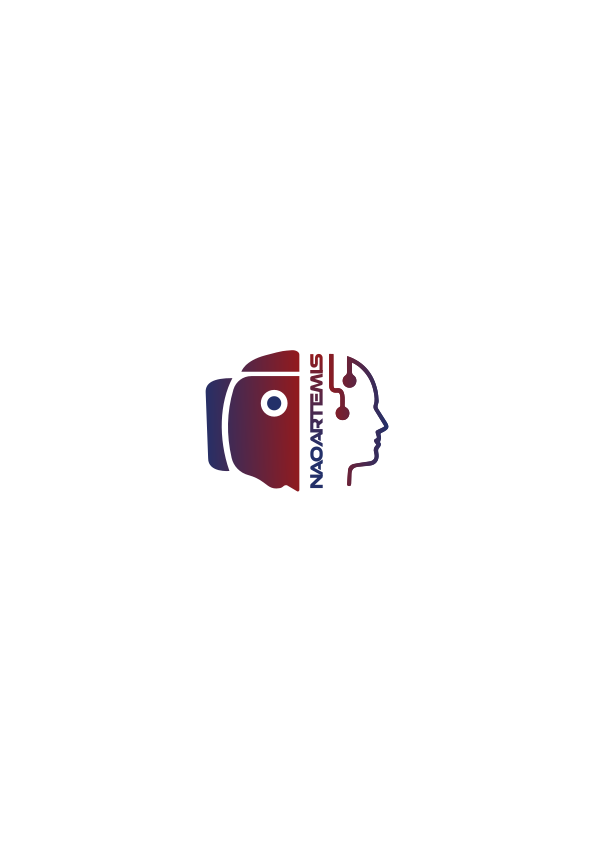
\includegraphics[width=0.2\textwidth]{figures/logo_v1.png}
    \caption{Logo versione 1}
    \label{fig:logo_v1}
\end{figure}

Questa versione \`e ottimizzata per l’uso come immagine profilo sulle piattaforme social (Instagram, Facebook, TikTok, YouTube). Grazie al formato verticale e alla composizione compatta, il logo mantiene chiarezza e riconoscibilit\`a anche in dimensioni ridotte. Il nome del progetto \`e integrato verticalmente tra la sagoma robotica e il volto umano.

\textbf{Logo 2 -- Merchandising e stampa (versione centrale)}\\
\begin{figure}[H]
    \centering
    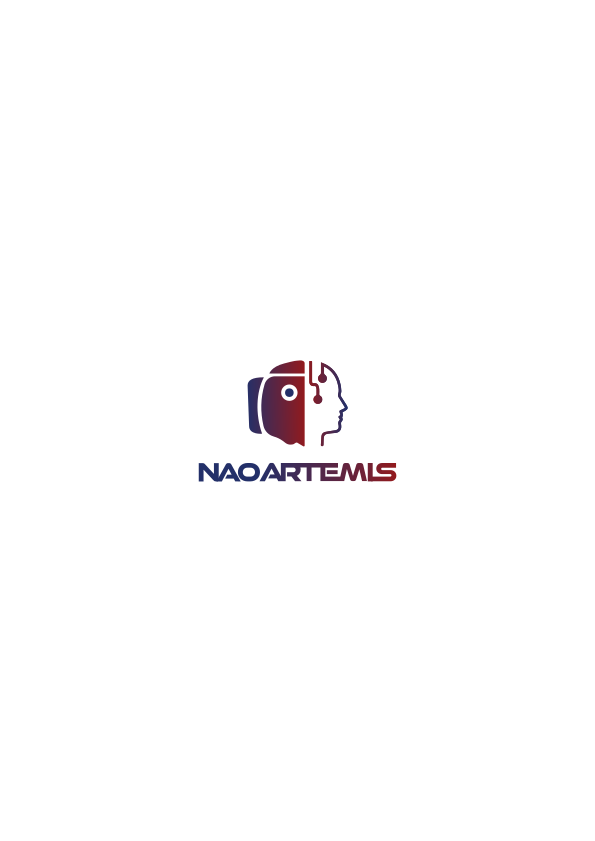
\includegraphics[width=0.3\textwidth]{figures/logo_v2.png}
    \caption{Logo versione 2}
    \label{fig:logo_v2}
\end{figure}
Questa variante, pensata per materiali stampati e fisici (magliette e biglietti da visita), presenta una composizione centrata e bilanciata tra il disegno e il nome del team. La disposizione orizzontale della scritta assicura leggibilit\`a immediata.

\textbf{Logo 3 -- Comunicazione ufficiale (versione estesa)}\\
\begin{figure}[H]
    \centering
    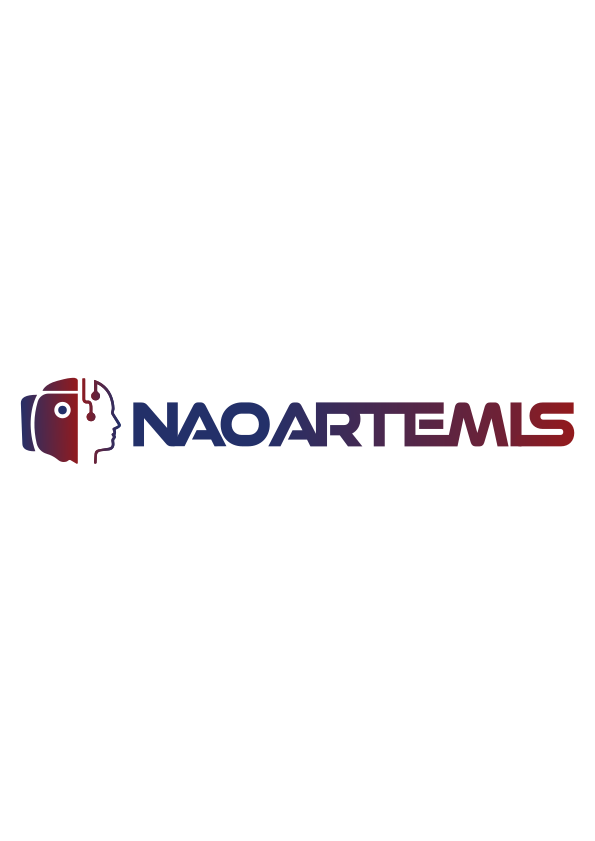
\includegraphics[width=0.5\textwidth]{figures/logo_v3.png}
    \caption{Logo versione 3}
    \label{fig:logo_v3}
\end{figure}
La terza versione \`e progettata per l’utilizzo in contesti digitali o editoriali in cui \`e importante valorizzare il nome del team. Con il testo “NAOARTEMIS” disposto in grande evidenza accanto all’icona composita, questo logo \`e stato impiegato per intestazioni di documenti e nel sito web.

La palette cromatica utilizza principalmente due colori: blu e rosso, talvolta sfumati come nel caso del logo. Le font scelte sono Montserrat e Good Timing. L’uniformit\`a visiva tra tutti i materiali (social, presentazioni, sito web) garantisce coerenza e riconoscibilit\`a al team.

\subsection{Presenza digitale: gestione strategica dei social media}
 La presenza online si \`e sviluppata su diverse piattaforme: Instagram, TikTok, Facebook, YouTube e LinkedIn, ciascuna con contenuti adattati al proprio pubblico di riferimento e con un piano editoriale condiviso.

\textbf{Instagram}\\
Su Instagram sono stati pubblicati post statici, caroselli e biografie per presentare il team, la scuola, gli obiettivi e i partner; descrizione del progetto suddivisa in post sequenziali; approfondimenti su sport, AI, inclusivit\`a, Audace, benessere e prestazione sportiva; stories dinamiche e reel tematici.

\begin{center}
    \includegraphics[width=0.4\textwidth]{figures/instagram.jpg}
\end{center}

\textbf{TikTok}\\
Sono stati pubblicati gli stessi reel di Instagram, adattati al formato della piattaforma. I contenuti hanno privilegiato velocit\`a, immediatezza e originalit\`a, per attrarre l’attenzione di un pubblico ancora pi\`u giovane.

\textbf{Facebook}\\
Contenuti condivisi con taglio pi\`u istituzionale, per raggiungere genitori, scuole e partner esterni.

\textbf{YouTube}\\
Raccolta di tutti i video pubblicati, pi\`u un video  completo per presentazioni ufficiali ed eventi.

\textbf{LinkedIn}\\
Utilizzato per la comunicazione tecnica e professionale con docenti e aziende.

Infine, è stato utilizzato Linktree, uno strumento utile in contesti professionali per organizzare e condividere in modo efficace una raccolta di link per gli acessi ai diversi social, attraverso un'unica pagina facilmente accessibile.

\begin{center}
    \includegraphics[width=0.4\textwidth]{figures/linktree.jpg}
\end{center}

\subsection{Piattaforma web: il sito ufficiale NaoArtemis}

 È stato realizzato un sito web dedicato al progetto \text{NaoArtemis}, sviluppato per la \text{NAO Challenge 2025}, al fine di documentare in modo strutturato e accessibile tutte le componenti principali dell’iniziativa. È  stata inserita una \text{descrizione tecnica del progetto}, articolata nei due task principali (ottimizzazione dell’allenamento sportivo e inclusione dei tifosi). Sono specificati i ruoli dei membri e la scuola di appartenenza. Vi è infine una sezione dedicata alla \text{collaborazione con la società sportiva Audace}.
\bigskip
\section{Membri del team e ruoli}

\subsection{Tecnologia, inclusione e scuola: il team NaoArtemis nasce alle Stimate}
Il team NaoArtemis nasce all'interno del Liceo “Alle Stimate” di Verona, un istituto con oltre due secoli di storia educativa, fondato nel 1816 da San Gaspare Bertoni. La scuola si distingue per il suo impegno nella formazione integrale della persona, che unisce l’eccellenza accademica alla promozione di valori umani, sociali e spirituali.

In questo contesto di apertura e innovazione, la scuola sostiene attivamente progetti interdisciplinari come la partecipazione alla NAO Challenge. Il team NaoArtemis, composto da studenti del liceo scientifico delle scienze applicate e guidato dal prof. Giovanni Bellorio, nasce proprio da questa visione educativa: coniugare passione per la tecnologia, spirito di squadra e impegno sociale.

\subsection{Divisione dei ruoli}
\textbf{Giovanni Bellorio} \\Docente di informatica, \`e il coach. Coordina gli incontri e gestisce gli aspetti organizzativi e amministrativi della NAO Challenge.

\textbf{Mattia Begali -- App developer} \\Responsabile dello sviluppo dell’app per Task 1. Lavora sulla programmazione e sull'integrazione dei sistemi intelligenti in Python.

\textbf{Laura Mascalzoni -- Social media manager e Team Leader} \\Coordina le piattaforme social, cura i contenuti multimediali e garantisce la coerenza comunicativa.

\textbf{Giacomo Santi -- Website developer} \\Responsabile del sito web ufficiale. Cura l'accessibilit\`a, l'aggiornamento e la presentazione tecnica del progetto.

\textbf{Alessandro Albertini -- Video content developer} \\Produce e monta i video. Gestisce la pipeline audiovisiva e l'adattamento ai diversi formati.

\textbf{Alessandra Fiornini -- Social media content developer} \\Supporta la comunicazione visiva e testuale sui social, mostrando precisione e cura.

\textbf{Haseeb Nabi -- Webapp developer} \\Programmatore avanzato del robot NAO. Lavora su Task 1, computer vision e Web App.

\textbf{Marco Tomazzoli -- Nao Programmer} \\Responsabile delle funzionalit\`a di Task 2. Sviluppa l'interazione tramite CAA e il riconoscimento dei simboli ArUco.


\begin{figure}[b]
    \centering
    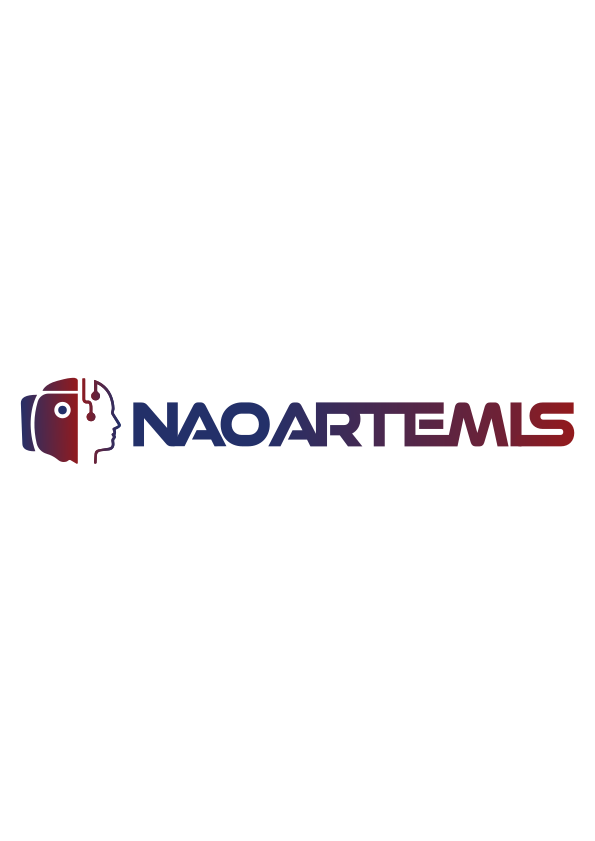
\includegraphics[scale=0.08]{figures/logo_v3.png}
    \label{fig:logo_con_scritta1}
\end{figure}


%\vspace{70pt}
%\listoffigures
\end{document}